\documentclass[t,12pt]{beamer}
\usepackage[utf8]{inputenc}
\usepackage[T1]{fontenc}
\usepackage{fancyhdr} % pour personnaliser les en-têtes
\usepackage{lastpage}
\usepackage[frenchb]{babel}
\usepackage{amsfonts,amssymb}
\usepackage{amsmath,amsthm}
\usepackage{paralist}
\usepackage{enumerate}
\usepackage{xspace}
\usepackage{xcolor}
\usepackage{variations}
\usepackage{xypic}
\usepackage{eurosym,multicol}
\usepackage{graphicx}
\usepackage[np]{numprint}
\usepackage{hyperref} 
\usepackage{setspace}
\usepackage{listings} % pour écrire des codes avec coloration syntaxique  

\usepackage{tikz}
\usetikzlibrary{calc, arrows, plotmarks,decorations.pathreplacing}
\usepackage{colortbl}
\usepackage{multirow}


\newtheorem{defi}{Définition}
\newtheorem{thm}{Théorème}
\newtheorem{thm-def}{Théorème/Définition}
\newtheorem{rmq}{Remarque}
\newtheorem{prop}{Propriété}
\newtheorem{cor}{Corollaire}
\newtheorem{lem}{Lemme}
\newtheorem{ex}{Exemple}
\newtheorem{cex}{Contre-exemple}
\newtheorem{prop-def}{Propriété-définition}
\newtheorem{exer}{Exercice}
\newtheorem{nota}{Notation}
\newtheorem{ax}{Axiome}
\newtheorem{appl}{Application}
\newtheorem{csq}{Conséquence}
%\def\di{\displaystyle}


\newcommand{\vtab}{\rule[-0.4em]{0pt}{1.2em}}
\newcommand{\V}{\overrightarrow}
\renewcommand{\thesection}{\Roman{section} }
\renewcommand{\thesubsection}{\arabic{subsection} }
\renewcommand{\thesubsubsection}{\alph{subsubsection} }
\newcommand{\C}{\mathbb{C}}
\newcommand{\R}{\mathbb{R}}
\newcommand{\Q}{\mathbb{Q}}
\newcommand{\Z}{\mathbb{Z}}
\newcommand{\N}{\mathbb{N}}



\usetheme{Warsaw}

\title{ 4 Questions sur les fonctions affines et les probabilités}
\author{Évaluation de 1 heure \\mercredi 25 mai 2022}
\date{Programme de révisions: Fonctions affines + Probabilités}
\begin{document}
	\maketitle	
\begin{frame}
	
	\frametitle{Question 1: }
Soient $F$ une fonction affine définie sur $\R$ et pour $a\in\R$ on considère le point $C\left(5;a\right)$.\hfill\\[0.3cm]

On sait que la courbe de la fonction $F$ passe par les points de coordonnées $A(-1;7)$ et $B(12;9)$. \hfill\\[0.3cm]
\begin{enumerate}
	\item Donner l'expression de la fonction $F$.
	\item Donner le tableau de signes de la fonction $F$.
	\item Donner la valeur de l'inconnue $a$ pour que le coefficient de la droite $\left(AC\right)$ soit égal à 5. 
\end{enumerate}
		

	

\end{frame}

\begin{frame}
	\frametitle{Question 2: }
		On lance une pièce truquée qui donne 8 fois plus de "Pile" que de "Face". 
		\begin{enumerate}
			\item Donner la loi de probabilité associée à cette expérience aléatoire.
			\item Compléter ce programme Python pour qu'il modélise le lancer de cette pièce truquée.  
		\end{enumerate}
	\begin{figure}
		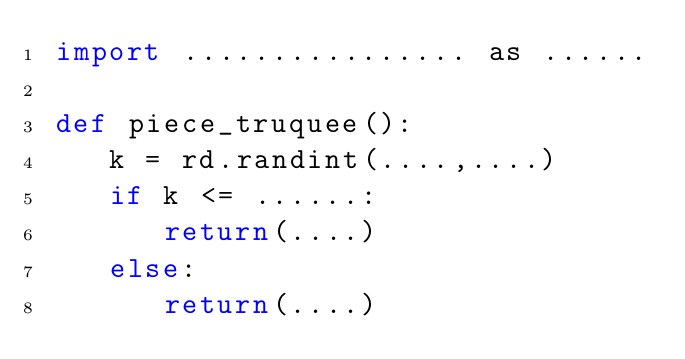
\includegraphics[scale=0.4]{1.png}
	\end{figure}
	



\end{frame}

\begin{frame}
	\frametitle{Question 3: }
	Soit $H$ une fonction affine définie sur $\R$. Soit $\alpha\in\R$ on considère le point $Z\left(\alpha ;6\right)$.\hfill\\[0.2cm]
	On sait que la courbe de la fonction $H$ passe par les points de coordonnées $X(8;7)$ et $Y(2;-9)$. \hfill\\[0.3cm]
	\begin{enumerate}
		\item Donner l'expression de la fonction $H$.
		\item Donner le tableau de variations de la fonction $H$.
		\item Donner la valeur de l'inconnue $\alpha$ pour que le coefficient de la droite $\left(YZ\right)$ soit égal à -3. 
	\end{enumerate}
	
	
	
\end{frame}

\begin{frame}
	
	\frametitle{Question 4: }
	On place dans un sac 6 billes noires, 12 billes vertes et 18 billes bleues. On effectue un tirage et on note la couleur de la bille à l'aide des nombres $\{0 ; 1 ; 2\}$ respectivement associés aux couleurs: noire, verte et bleu. 
	\begin{enumerate}
		\item Donner la loi de probabilité associée à cette expérience aléatoire et compléter cette fonction en langage Python pour qu'elle modélise cette expérience aléatoire. 
	\end{enumerate}

	\begin{figure}
		\centering
		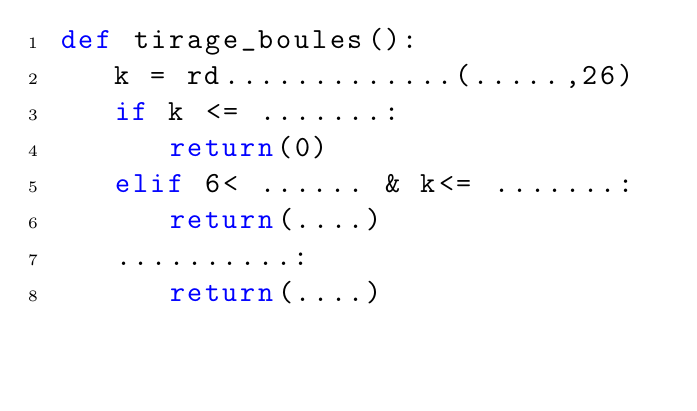
\includegraphics[scale=0.37]{2.png}
	\end{figure}


	
\end{frame}




\end{document}